\section{Semaine 2 : 13/02/2023 - 17/02/2023}
\graphicspath{{semaines/semaine_2/images/}}

\begin{abstract}
	(Les résultats en semaine 1 ont été obtenus en début de semaine.)
	
	Après la semaine dernière, on s'est dit qu'une bonne idée serait de prendre une solution manufacturée (analytique) afin de pouvoir comparer les erreurs avec FEM classique, PhiFEM, le FNO et le FNO+correction. On a choisi de prendre $u$ comme une gaussienne et ainsi le f associé. Attention, il a fallut normaliser les F pour le FNO. On a également eut l'idée d'utiliser une solution sur-raffinée (à la place d'une solution exacte) mais ça n'a pas encore été testé.
\end{abstract}

\subsection{Génération de données}

On considère toujours $\Omega$ le cercle de rayon $\sqrt{2}/4$ et de centre $(0.5,0.5)$ avec $\Phi(x,y)=-1/8+(x-1/2)^2+(y-1/2)^2$ et le domaine fictif $O=(0,1)^2$ (\href{https://colab.research.google.com/drive/1Ymb1XZU80fwy7XxkL5_SsNs-ZVIVs3dm#scrollTo=GYtkSETwcBRp}{"DataGen\_PhiFEM\_u\_gaussienne"}).

On souhaite résoudre 
\begin{equation*}
	\begin{cases}
		-\Delta u &= f\,, \quad \text{dans $\Omega$}\,, \\
		u &= g\,, \quad \text{sur $\Gamma$}\,, \\
	\end{cases}
\end{equation*}

Notre solution analytique est
$$u_{ex}(x,y) = \exp\left(-\frac{(x-\mu_0)^2 + (y-\mu_1)^2}{2\sigma^2}\right)\,, $$ 
avec $\sigma \sim \mathcal{U}([0.1,0.6])$ et $\mu_0, \mu_1 \sim \mathcal{U}([-0.9, 0.9])$.

Ainsi 
$$f(x,y)=\left(\frac{2\sigma^2-(x-\mu_0)^2-(y-\mu_1)^2}{\sigma^4}\right)*\exp\left(-\frac{(x-\mu_0)^2 + (y-\mu_1)^2}{2\sigma^2}\right)$$
et
$$g(x,y)=u_{ex}(x,y)$$

Pour l'apprentissage du FNO, on va normaliser $f$ par $\max_f ||f||_{L^2(\Omega_h)}$

\textbf{Formulation faible :}

On utiliser une méthode directe pour inclure les conditions de Dirichlet homogène :

$$\int_{\Omega_h}\nabla(\bar{\phi}w)\nabla(\bar{\phi}v)-\int_{\partial\Omega_h}\frac{\partial}{\partial n}(\bar{\phi}w)\bar{\phi}v+G_h(w,v)=\int_{\Omega_h}f\bar{\phi}v-\left(\int_{\Omega_h}\nabla(g)\nabla(\bar{\phi}v)-\int_{\partial\Omega_h}\frac{\partial g}{\partial n}\bar{\phi}v\right)+G_h^{rhs}(v)$$
avec
$$G_h(w,v)=\sigma h\sum_{E\in\mathcal{F}_h^\Gamma}\int_E\left[\frac{\partial}{\partial n}(\bar{\phi}w)\right]\left[\frac{\partial}{\partial n}(\bar{\phi}v)\right]+\sigma h^2\sum_{T\in\mathcal{T}_h^\Gamma}\int_T \Delta(\bar{\phi}w)\Delta(\bar{\phi}v)$$
et
$$G_h^{rhs}(v)=-\sigma h^2\sum_{T\in\mathcal{T}_h^\Gamma}\int_T f\Delta(\bar{\phi}v)-\sigma h\sum_{E\in\mathcal{F}_h^\Gamma}\int_E\left[\frac{\partial g}{\partial n}\right]\left[\frac{\partial}{\partial n}(\bar{\phi}v)\right]-\sigma h^2\sum_{T\in\mathcal{T}_h^\Gamma}\int_T \Delta(g)\Delta(\bar{\phi}v)$$

\subsection{Résultat}

Voici un exemple de résultats obtenu sur $u$ une gaussienne (\href{https://colab.research.google.com/drive/1kcxNffAI2-fqmWv9swLnUrKGJRopedxF#scrollTo=oSFmuK2uVCXX}{"phifem\_u\_gaussienne"}).

\begin{minipage}{\linewidth}
	\centering
	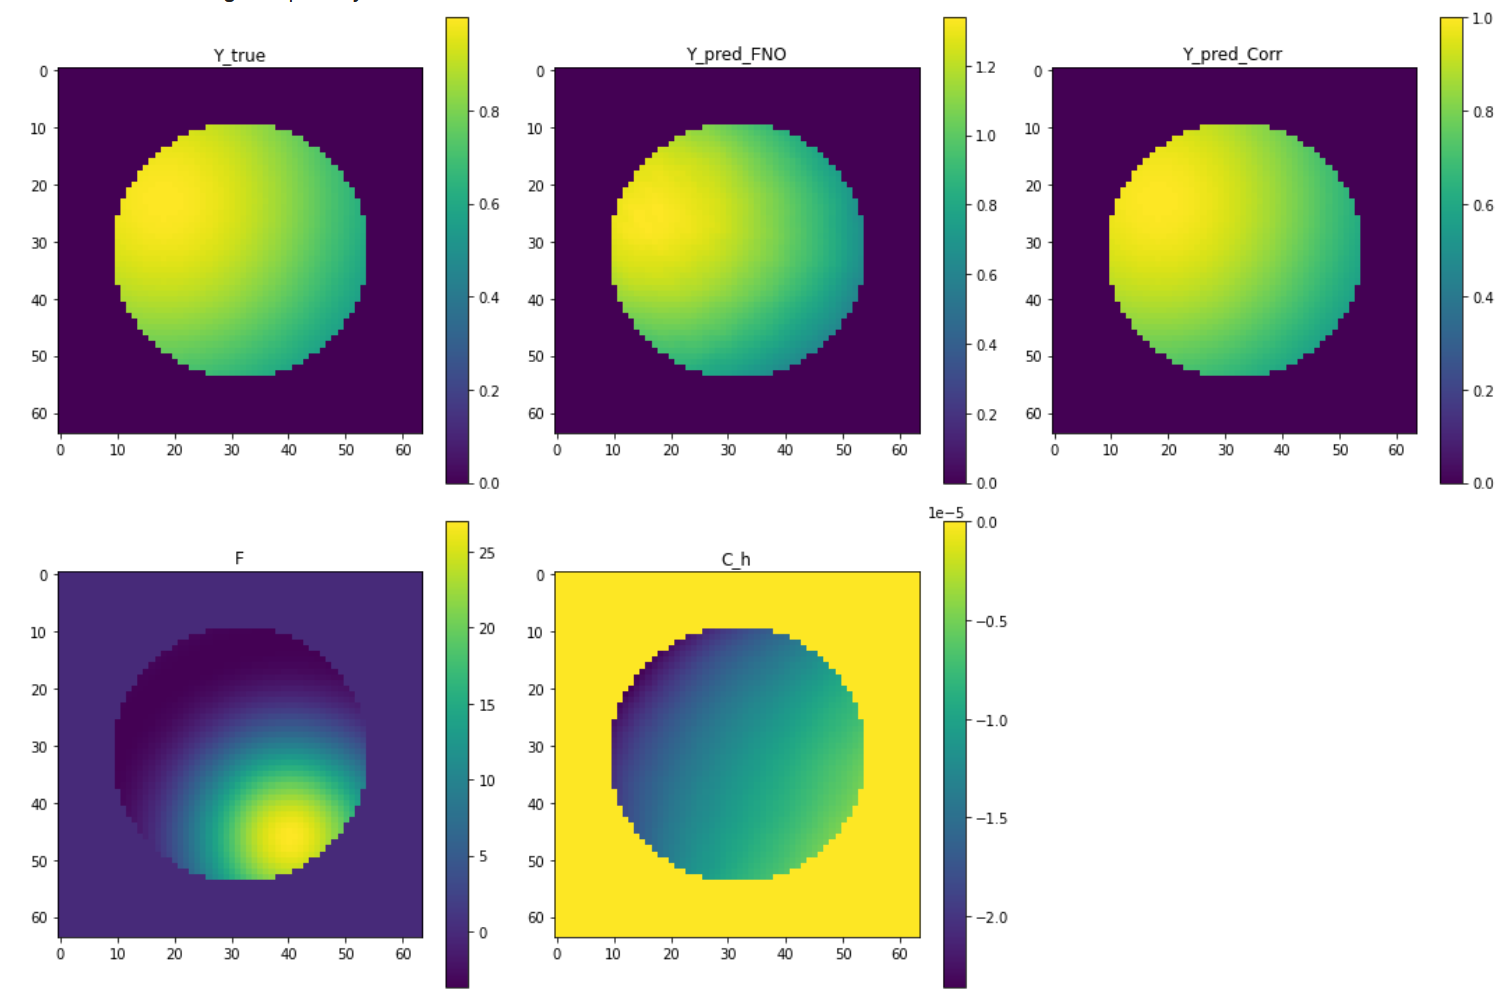
\includegraphics[width=0.45\linewidth]{resultat.png}
\end{minipage}

\conclusion{C'est en fin de semaine qu'on s'est rendue compte du problème du FNO : qu'il faut retourner $w$ et pas $u$. Les modifications ont été faites mais les résultats ne semblent toujours pas convaincant (résultats supprimés malencontreusement).
	
En fait, on a remarqué que prendre $g=u_{ex}$ sur $\Omega$ entier posait problème pour la correction, car on obtient $w=0$ et donc le problème de correction n'a plus de sens. Une solution à celà a été proposé par Emmanuel : il faudrait prendre $g=u_{ex}$ sur $\Gamma$ et étendre la solution (par exemple en utilisant un nouveau réseau de neurones qui nous fournirait une solution lisse). Mais pour l'instant, on va simplement choisir une autre solution analytique, où on n'est pas obligé de prendre $g=u_{ex}$ sur tout le domaine.

On a également eut l'idée de se ramener à un problème homogène (passage du problème en $f$ au problème en $\tilde{f}=f+\Delta g$)

Un autre problème constaté est qu'il faut utilisé le $\phi$ initial pour la génération des espaces $\mathcal{F}_h^\Gamma$ et $\mathcal{T}_h^\Gamma$.}